% =============================================================================
% COPYRIGHT AND DISCLAIMER
% =============================================================================
% This file is provided as a convenience template for competition participants.
% By using it, you accept full responsibility for compliance with all applicable
% copyright, licensing, and usage rules of the Association for Computing
% Machinery (ACM) and of any LaTeX packages you load (including, without
% limitation, the "acmart" document class and related ACM materials).
%
% Consult ACM's official publication, template, and copyright policies before
% using this setup for any purpose other than this competition. Do not assume
% that this template may be reused, redistributed, or submitted elsewhere
% without independently verifying ACM's current rules.
%
% Use of the "acmart" class, the "sigconf" option, or ACM-style formatting in
% this template does NOT mean that this report, this competition, its organizers,
% or any resulting PDF is sponsored, endorsed, affiliated with, or published by
% ACM. ACM trademarks and branding remain the property of ACM.
%
% Template packages live in preamble.tex.
% Citations live in main.bib. Edit this file with your paper content.
% =============================================================================

\documentclass[sigconf]{acmart}
% Reconstruction of the template's preamble.tex (the original was not available); settings inferred from the template PDF
\setcopyright{none}
\settopmatter{printacmref=false}
\copyrightyear{2026}
\acmConference[Kaggle Competition]{Solar Filament Segmentation Challenge 2026}{2026}{kaggle.com/competitions/filament-segmentation-2026}
\acmYear{2026}
\acmDOI{}
\acmISBN{}
\newif\ifguideStyle
\newcommand{\guide}[1]{\ifguideStyle{\color{gray!65}\itshape #1}\fi}


% Guide styling: \guideStyletrue = show gray italic hints; \guideStylefalse = omit them
% \guideStyletrue
\guideStylefalse

\begin{document}

\title[Learning from Disagreeing Annotators]{Learning from Disagreeing Annotators: Soft-Label U-Net Ensembles with PQ-Tuned Post-Processing}  % Replace this with your title
\subtitle{A Solution to the Solar Filament Segmentation Challenge 2026} % DO NOT CHANGE


\author{Johnson Chishimba}
\affiliation{%
  \city{Sapporo}
  \state{Hokkaido}
  \country{Japan}
}
\email{johnson.mapalo@gmail.com}   % <- Replace with your own email

\begin{abstract}
    This report describes our solution to the Solar Filament Segmentation Challenge~2026, a Kaggle competition on automatic segmentation of solar filaments in GONG H-$\alpha$ observations. The training labels are noisy: 42\% of the 707 training images were labelled by two or three annotators, who agree with each other at a Panoptic Quality (PQ) of only 0.34. We therefore train a U-Net with a ResNet34 encoder on the fraction of annotators who marked each pixel, segment the whole solar disk at $1024\times1024$ pixels in one pass, average five cross-validation models with flip test-time augmentation, and form filament instances with a post-processing step whose five settings are tuned for PQ on out-of-fold predictions. Out of fold, the method reaches PQ 0.408 against each annotator (0.353 with all annotators of an image pooled), above human agreement, and it scores 0.36 on the public leaderboard. A larger encoder, model averaging and a learned instance score each change PQ by less than 0.005, within the uncertainty of the comparison; most of the remaining error is a 1--2 pixel boundary disagreement that the annotators share.
\end{abstract}

\maketitle

\ifguideStyle
\noindent{\color{gray!65}\itshape
Guide mode is on.}
\par\medskip
\fi


% ==================================== %
%              INTRODUCTION            %
% ==================================== %
\section{Introduction}
    This report goes over the details of our submitted solution to the Solar Filament Segmentation Challenge~2026 \cite{filament-segmentation-2026}. The challenge, launched on July~10,~2026, is organized by the Earth-Space AI Research (ESAIR) Lab\footnote{\href{https://www.esairlab.com/home}{www.esairlab.com/}}. This challenge utilizes the MAGFiLO dataset for evaluation of the segmentation algorithms \cite{ahmadzadeh2024dataset}. Our solution treats the disagreement between annotators as the central property of the data. A whole-disk U-Net is trained on soft labels, five cross-validation models are averaged, and filament instances are formed by a post-processing step tuned directly for PQ~\cite{kirillov2019panoptic}. Section~\ref{sec:methodology} describes the pipeline (Fig.~\ref{fig:pipeline}) and the data properties behind each choice; Section~\ref{sec:evaluation} reports out-of-fold results with uncertainty, ablations, run time, and an analysis of the remaining error. Code, the five trained models and a notebook that reproduces the submission are at \url{https://github.com/Mapalo90/competition}.


% ==================================== %
%              METHODOLOGY             %
% ==================================== %
\section{Methodology}\label{sec:methodology}

\begin{figure*}[t]
  \centering
  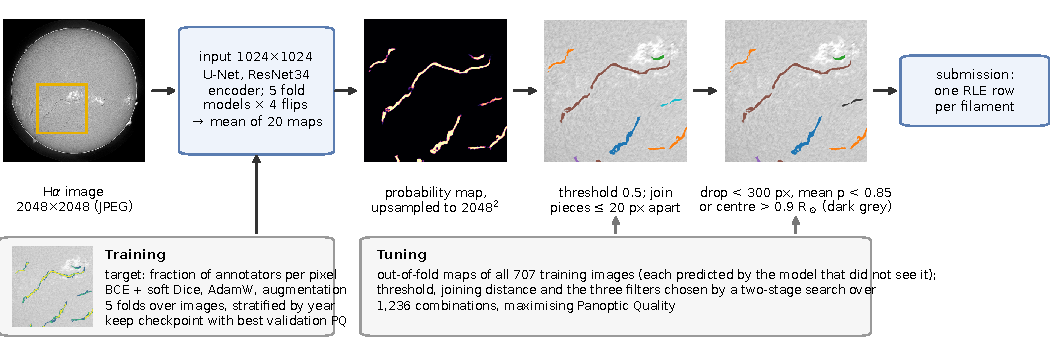
\includegraphics[width=\textwidth]{figures/pipeline}
  \caption{The pipeline, illustrated on training image 20140216230134Lh (three annotators, out-of-fold prediction). Each image is resized to $1024\times1024$ and segmented by five fold models with four flips each; the mean probability map is upsampled to full resolution, thresholded, nearby pieces are joined into one filament (the long brown filament is three pieces), and weak, small or limb candidates are dropped (dark grey). The thumbnails show the $700\times700$ px region boxed on the disk. Training uses soft targets (colour: fraction of the three annotators); all post-processing settings are tuned on out-of-fold maps.}
  \label{fig:pipeline}
\end{figure*}

\subsection{Data and splits}
We use only the H-$\alpha$ images and the segmentation masks of the training set: 707 images of $2048\times2048$ pixels with 1{,}154 annotation sets (one per annotator and image) and 8{,}199 filaments. The test set has 180 images and is used only for inference. Four properties of the data shaped the design.
(i)~\emph{Annotators disagree.} 296 images (42\%) carry two or three independent annotation sets. Scored against each other, annotators agree at PQ 0.340 (95\% interval 0.324--0.356, 598 pairs), and their filament counts on the same image range from 0.67 to 1.33 times the image average (10th--90th percentile). Any single annotation is therefore a noisy target.
(ii)~\emph{Instances are nearly connected regions.} 99.6\% of labelled filaments rasterise to one connected region and only 2.9\% have a neighbour within 10\,px, but annotators draw a filament broken by faint gaps as one object.
(iii)~\emph{Boundaries matter more than resolution.} Filaments are typically 8\,px wide (median area 1{,}228\,px). Resizing a label to 1024\,px and back keeps a median IoU of 0.98, whereas eroding it by one pixel drops the median IoU to 0.71 and pushes 6\% of filaments below the 0.5 IoU needed for a match.
(iv)~\emph{Position.} 99\% of labelled filament centres lie within 0.9 solar radii ($R_\odot$), and 14\% of images show a faint off-disk halo that misleads threshold-based disk detection by up to 120\,px.

Training and test images cover the same years and observing sites (35\% of test images were taken within a day of a training image), so we split over images rather than time: five folds stratified by year, with all annotation sets of an image in the same fold (142, 142, 141, 141 and 141 images). Each fold model is trained on four folds and predicts the fifth, so every training image receives an \emph{out-of-fold} (OOF) prediction from the one model that never saw it. All model selection and tuning use these OOF predictions only.

\subsection{Network and training}
The network is a U-Net~\cite{ronneberger2015unet}: an encoder that downsamples the image to coarse, semantically rich features, and a decoder that upsamples them back to full resolution, with skip connections that carry fine spatial detail across. The encoder is a ResNet34~\cite{he2016resnet} pretrained on ImageNet~\cite{deng2009imagenet}, adapted to one input channel (segmentation-models-pytorch~\cite{iakubovskii2019smp}); the decoder outputs one logit per pixel. Images are resized to $1024\times1024$ with area interpolation and normalised; no other preprocessing is applied, so the network sees the limb and the off-disk background and learns to ignore them. ImageNet pretraining of the encoder is the only external resource, and no annotation metadata other than the masks (spines, bounding boxes, chirality) is used. The target is the fraction of the image's annotators who marked each pixel ($0$, $\frac13$, $\frac12$, $\frac23$ or $1$), so the network learns how likely a pixel is to be labelled rather than one annotator's style. The loss is binary cross-entropy plus soft Dice~\cite{milletari2016vnet}. We train with AdamW~\cite{loshchilov2019adamw} (learning rate $3\times10^{-4}$, weight decay $10^{-4}$, one warm-up epoch, cosine decay), batches of 8 and mixed precision, augmenting with random dihedral flips, rotation ($\pm45^\circ$), scaling ($\pm5\%$), brightness, contrast and gamma changes, blur and noise. Each fold trains for 30 epochs (40 for fold~0). Every 10 epochs (5 for fold~0) the validation PQ is computed and the best checkpoint, by PQ rather than by loss, is kept.

\subsection{Inference and instance extraction}
At test time each fold model predicts the image and its three flips, and the 20 probability maps are averaged and upsampled to $2048\times2048$. Instances are then formed in three steps (Fig.~\ref{fig:pipeline}). \emph{Threshold:} pixels with probability $\geq0.5$ form candidate regions. \emph{Join:} regions at most 20\,px apart become one filament, without painting the gap: the mask is dilated with a disk of radius 10\,px, and each connected region of the dilated mask collects the original pixels inside it. This mimics how annotators label fragmented filaments. \emph{Filter:} filaments smaller than 300\,px, with mean probability below 0.85, or with their centroid beyond $0.9\,R_\odot$ are removed. The disk centre and radius come from a least-squares circle through the steepest brightness drop along 180 rays from a rough centre, refitted after discarding outliers, which the halo does not disturb. Every remaining filament becomes one row of the submission, encoded as COCO run-length; instances cannot overlap by construction. The threshold, joining distance and the three filter values were chosen by a two-stage search over 1{,}236 combinations, maximising PQ on the OOF maps of all 707 training images: first the threshold and filters without joining, then the joining distance and threshold around the best result.

\begin{figure*}[t]
  \centering
  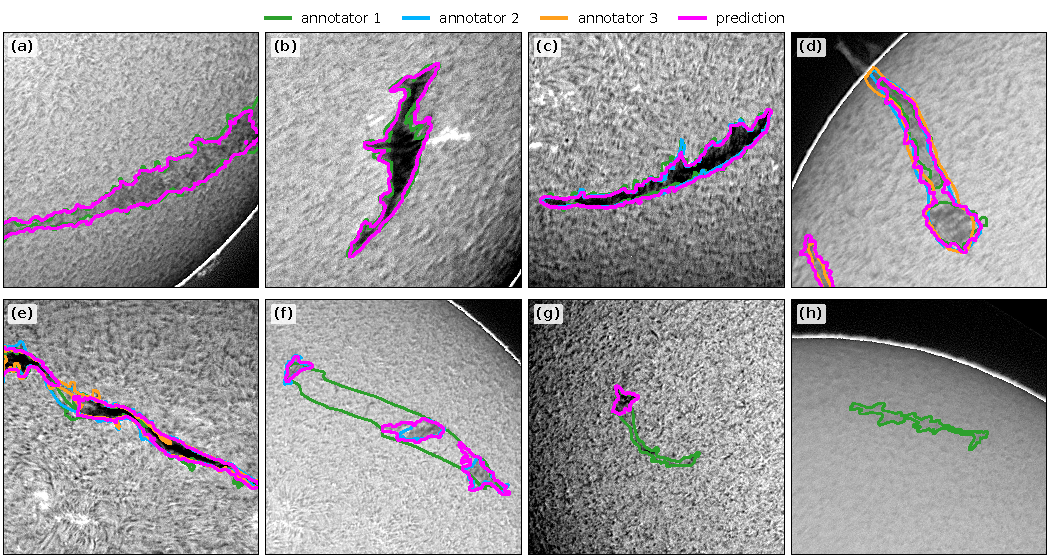
\includegraphics[width=\textwidth]{figures/examples}
  \caption{Out-of-fold predictions (magenta) and annotator outlines on $512\times512$ px crops of training images. Top: (a)~a large faint filament (IoU 0.73 with the label); (b)~a dark filament with barbs; (c)~two annotators who agree; (d)~three annotators near the limb. Bottom: (e)~three annotators who disagree on the extent; (f)~annotator~1 outlines a faint envelope that annotator~2 and the model restrict to its dark cores; (g)~a faint tail is missed, so the match fails (IoU $<0.5$); (h)~a low-contrast image in which nothing is detected.}
  \label{fig:examples}
\end{figure*}


% ==================================== %
%              EVALUATION              %
% ==================================== %
\section{Evaluation}\label{sec:evaluation}

\subsection{Strategy}
We score the OOF predictions of all 707 training images with $\mathrm{PQ}=\sum_{\text{matches}}\mathrm{IoU}\,/\,(\mathrm{TP}+\frac12\mathrm{FP}+\frac12\mathrm{FN})=\mathrm{SQ}\times\mathrm{RQ}$, where a prediction and a labelled filament match if their IoU exceeds 0.5. With several annotators per image, PQ can be computed against each annotator's set separately and summed (as in the organizers' self-evaluation notebook; ``each annotator'' below) or against all annotators' filaments pooled in one list with one-to-one matching (``pooled''); we report both. Uncertainty is given as 95\% percentile-bootstrap intervals over images (10{,}000 resamples) and as the spread over folds. Human agreement on the same images, one annotator scored against another, is the reference point.

\begin{table}[t]
  \caption{Out-of-fold results on all 707 training images (95\% bootstrap intervals over images), human agreement, and the public leaderboard.}
  \label{tab:main}
  \small
  \begin{tabular}{@{}lcccc@{}}
    \toprule
    & PQ & 95\% interval & SQ & RQ \\
    \midrule
    OOF, each annotator & \textbf{0.408} & 0.399--0.418 & 0.668 & 0.611 \\
    OOF, annotators pooled & 0.353 & 0.344--0.363 & 0.681 & 0.519 \\
    OOF, threshold 0.5 only & 0.331 & & & \\
    Human: annotator vs.\ annotator & 0.340 & 0.324--0.356 & 0.634 & 0.536 \\
    Public leaderboard ($\approx$90 images) & 0.36 & $\pm0.024^a$ & & \\
    \bottomrule
  \end{tabular}\\[2pt]
  {\footnotesize Folds 0--4, each annotator: 0.427, 0.405, 0.391, 0.409, 0.409 (mean 0.408, s.d.\ 0.013). $^a$Two standard deviations of PQ over random sets of 90 OOF images.}
\end{table}

\subsection{Results}
Table~\ref{tab:main} summarises the OOF results. The model exceeds human agreement by 0.07 PQ, and the five folds lie within $\pm0.02$ of the mean. Tuned post-processing adds 0.077 over plain thresholding: 0.073 from the filters and 0.004 from joining, which reduces the number of labelled filaments split into several predictions from 469 to 323. Fig.~\ref{fig:dist} shows the distributions named in the evaluation rubric: the IoU and Dice of every overlapping pair of labelled and predicted filaments, and the one-to-many and many-to-one relations. 76\% of labelled filaments overlap exactly one prediction and 83\% of predictions overlap exactly one labelled filament; about 4\% overlap two or more. Fig.~\ref{fig:sens} shows that PQ is flat around the chosen settings except for the mean-probability filter, which costs PQ quickly above 0.85; the result therefore does not depend on a finely tuned value. Fig.~\ref{fig:examples} shows typical predictions: they follow the dark body of each filament closely and stop where the contrast fades, including at barbs.

\begin{figure}[t]
  \centering
  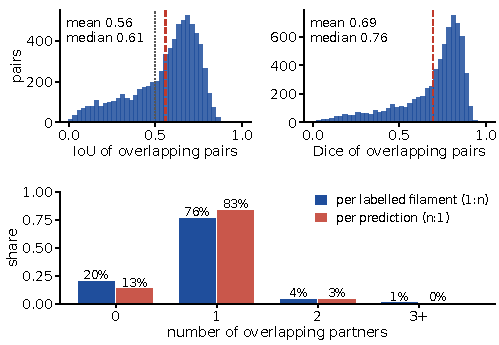
\includegraphics[width=\columnwidth]{figures/distributions}
  \caption{All 707 training images (out of fold), final settings: IoU and Dice of every overlapping (label, prediction) pair, and how many predictions each labelled filament overlaps (1:n) and vice versa (n:1).}
  \label{fig:dist}
\end{figure}

\begin{figure}[t]
  \centering
  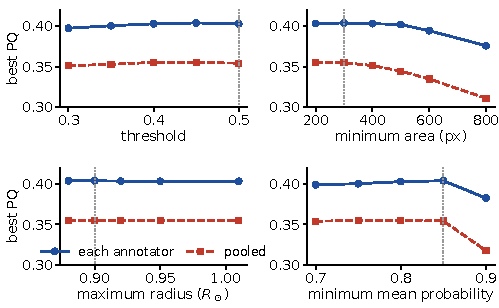
\includegraphics[width=\columnwidth]{figures/sensitivity}
  \caption{Best OOF PQ (707 images, before joining) for each value of one post-processing setting, with the other settings free. Dotted lines mark the final settings.}
  \label{fig:sens}
\end{figure}

\begin{table}[t]
  \caption{Ablations on fold 0 (142 images), PQ against each annotator with 95\% bootstrap intervals, and the paired difference to the reference model. Costs are relative to the reference.}
  \label{tab:abl}
  \small
  \setlength{\tabcolsep}{3.2pt}
  \begin{tabular}{@{}lccc@{}}
    \toprule
    Variant & PQ & $\Delta$ PQ & train / infer \\
    \midrule
    ResNet34, $1024^2$ (ref.) & 0.427 {\scriptsize[.409, .445]} & -- & 1 / 1 \\
    ResNet34, $768^2$ crops & 0.420 {\scriptsize[.402, .438]} & $-$0.007 {\scriptsize[$-$.014, .001]} & 0.6 / 1 \\
    ResNet50, $768^2$ crops & 0.426 {\scriptsize[.409, .443]} & $-$0.001 {\scriptsize[$-$.010, .007]} & 1.0 / 1.7 \\
    Ref.\ + ResNet50 average & 0.430 {\scriptsize[.413, .448]} & $+$0.004 {\scriptsize[$-$.002, .009]} & 2.0 / 2.7 \\
    \bottomrule
  \end{tabular}
\end{table}

\subsection{Ablations and run time}
Table~\ref{tab:abl} varies the model while keeping the post-processing fixed. A ResNet50 encoder needs $768\times768$ crops to fit two 16\,GB GPUs and only matches the ResNet34 reference, at 1.7 times its inference cost; averaging the two architectures gains 0.004, and every difference lies inside its 95\% interval. Two post-processing variants also stayed within noise: a learned per-filament keep/drop score (gradient-boosted trees on 23 shape, probability and position features, cross-validated by image) gained 0.004 against each annotator and nothing under pooled scoring, and recalibrating the threshold for averaged maps gained at most 0.003. We kept the simpler, cheaper configuration.
Training takes about 2.3 minutes per epoch, about 70 minutes per fold, on two NVIDIA T4 GPUs. Inference costs about 0.8\,s per image and model with test-time augmentation (about 4\,s for the five-model ensemble), plus 0.2\,s of post-processing on one CPU core.
\emph{Reproducibility.} The repository holds the five models (float16, 49\,MB each) and a notebook that rebuilds everything from them and the competition data. Re-run on Kaggle, it reproduced the OOF results above and the submitted file: 1{,}150 of its 1{,}152 filaments with mean IoU 0.9998 (PQ 0.999 against the submitted file); the other two have a mean probability of 0.850, exactly at the filter threshold.

\begin{figure}[t]
  \centering
  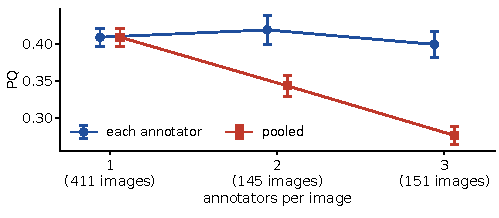
\includegraphics[width=\columnwidth]{figures/by_annotators}
  \caption{PQ by number of annotators per image, all 707 training images (out of fold), with 95\% bootstrap intervals. Against each annotator PQ hardly depends on how many people labelled the image; pooled PQ falls with every additional annotator.}
  \label{fig:byann}
\end{figure}

\subsection{Strengths, weaknesses and possible improvements}
\emph{Strengths.} The method exceeds human agreement out of fold with a single standard architecture, needs no tiling, runs in about 4\,s per image, and its post-processing settings sit on a plateau rather than a sharp optimum. The disk fit makes the limb filter safe on halo images, and the soft targets make the model robust to which annotator labelled an image: PQ against each annotator is 0.410, 0.420 and 0.400 for images with one, two and three annotators, with overlapping intervals (Fig.~\ref{fig:byann}).

\emph{Scoring rule.} Pooled PQ is not just lower but falls with every additional annotator (0.410, 0.344 and 0.276), because a filament drawn by three annotators appears three times in the pooled list and a non-overlapping prediction can match only one copy. The public leaderboard (0.35--0.36) is consistent with our pooled estimate (0.353) rather than the per-annotator one (0.408). Re-tuning for the pooled rule keeps slightly more filaments (6.8 instead of 6.6 per image on fold~0) and gains 0.003, below what the leaderboard can resolve.

\emph{Weaknesses.} For matched pairs on fold~0, 53\% of missed labelled pixels lie in the outer 2\,px of a filament's body and 61\% of extra predicted pixels lie within 2\,px outside the label, so boundary placement, where annotators also disagree (Fig.~\ref{fig:examples}e,f), dominates the remaining loss. Thin structures narrower than 5\,px (barbs and threads) are only 2.4\% of the labelled area; within detected filaments the model captures 45\% of them versus 81\% of other filament pixels, and capturing all of them would raise SQ by at most 0.016. The missed barbs are essentially absent from the probability map (median probability 0.008, the same as unlabelled pixels beside the filament). An image-guided refinement that re-decides a thin band around each filament by local darkness raised the share of labelled thin parts covered from 35.5\% to 40.3\% but changed PQ by $-0.007$ to $+0.001$ ($-0.001$ on a held-out half), so we did not adopt it. Faint filaments in low-contrast images are missed (Fig.~\ref{fig:examples}g,h). Finally, the settings were tuned on the same OOF predictions they are scored on, so the OOF PQ is slightly optimistic, and the leaderboard's rule for multiply-annotated images is inferred rather than documented.

\emph{Possible improvements.} Modelling each annotator explicitly (for example, one output per annotator with a learned consensus), a boundary-aware loss, contrast normalisation per observing site for faint images, and a full-resolution refinement stage for thin structures address the weaknesses above; our ablations suggest these, rather than larger encoders, are where further gains lie.


% ==================================== %
%            ACKNOWLEDGMENT            %
% ==================================== %
\section{Acknowledgment}\label{sec:acknowledgment}
    % Do not change
    The organization of the Filament Segmentation Challenge 2026 is partially supported by the U.S. National Science Foundation (NSF) under Grant No. 2209912 and 2433781, directorate for Computer and Information Science and Engineering (CSE), and Office of Advanced Cyberinfrastructure (OAC), and Grant No. 2511630, AST Division Of Astronomical Sciences and MPS Directorate for Mathematical and Physical Sciences.

    The Filament Segmentation Challenge 2026 is sponsored by the U.S. National Science Foundation (NSF) National Solar Observatory (NSO). 

    This work utilizes GONG data obtained by the NSO Integrated Synoptic Program, managed by the National Solar Observatory, which is operated by the Association of Universities for Research in Astronomy (AURA), Inc. under a cooperative agreement with the National Science Foundation and with contribution from the National Oceanic and Atmospheric Administration. The GONG network of instruments is hosted by the Big Bear Solar Observatory, High Altitude Observatory, Learmonth Solar Observatory, Udaipur Solar Observatory, Instituto de Astrofísica de Canarias, and Cerro Tololo Interamerican Observatory.

\bibliographystyle{ACM-Reference-Format}
\bibliography{main}

\end{document}
